\documentclass[10pt]{report}

\usepackage{stan-talks}

\begin{document}
\sf%
\vspace*{-2pt}
% 
\noindent
\spc{\Huge\bfseries \color{MidnightBlue}{Stan}}
\\[8pt]
\spc{\Large\bfseries \color{MidnightBlue}{Statistical Inference Made Easy}}
\\[10pt]
\noindent
\spc{\slshape Core Development Team 
\hfill {\small (20 people, $\sim$4 FTE)}}
\\[2pt]
\spc{\footnotesize Andrew Gelman, \  Bob Carpenter, \
  Matt Hoffman, \ Daniel Lee, }
\\
\spc{\footnotesize Ben Goodrich, \  Michael Betancourt, \ Marcus
  Brubaker, \   Jiqiang Guo, }
\\
\spc{\footnotesize Peter Li, \ Allen Riddell, \  Marco Inacio, \ Jeffrey Arnold, }
\\
\spc{\footnotesize Mitzi Morris, \ Rob Trangucci, \ Rob Goedman, \
Brian Lau, }
\\
\spc{\footnotesize Jonah Sol Gabray, \ Alp Kucukelbir, \ Robert
  L.~Grant, \ Dustin Tran}
\\[-12pt]
\vfill
\hspace*{3pt}{\footnotesize Stan 2.7.0 \ \footnotesize (July 2015) 
\hfill \url{http://mc-stan.org}}
\hfill 
\includegraphics[width=0.4in]{img/new-logo.png}

% SECOND TITLE

\clearpage
\sf
\vspace*{6pt}
\noindent
\spc{\huge\bfseries \color{MidnightBlue}{Section 1.}}
\\[8pt]
\spc{\Huge\bfseries \color{MidnightBlue}{Bayesian Inference}}
\vfill
\noindent
\spc{\large\bfseries Bob Carpenter}
\\[4pt]
\spc{Columbia University}
\vfill
\hfill 
 
% \sld{Where is the Talk?}
% \begin{center}
% \vfill
% {\large\tt\bfseries
% http://mc-stan.org/bayes-mcmc.pdf
% }
% \vfill
% \end{center}

\mypart{Breaking News}

\sld{Stan Accepted on CRAN}
\begin{itemize}
\item Yeah!
\end{itemize}

\mypart{Warmup Exercise I}{Sample Variation}


\sld{Repeated i.i.d. Trials}

\noindent
\begin{minipage}[t]{0.69\textwidth}
\vspace*{-1.9in}
\begin{itemize}
\item Suppose we repeatedly generate a random outcome from among
several potential outcomes
\item Suppose the outcome chances are the same each time
\begin{subitemize}
\item i.e., outcomes are independent and identically distributed (i.i.d.)
\end{subitemize}
\item For example, spin a fair spinner (without cheating), such as one from \emph{Family Cricket}.
\end{itemize}
\end{minipage}
%
\begin{minipage}[t]{0.29\textwidth}
\hfill 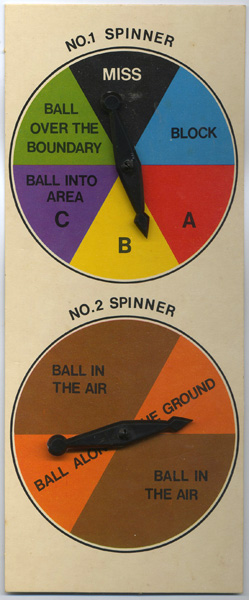
\includegraphics[height=2in]{img/family-cricket-spinner.jpg}
\end{minipage}
\vfill
\hfill {\tiny Image source: \url{http://replaycricket.com/2010/10/29/family-cricket/}}

\sld{Repeated i.i.d. Binary Trials}
\begin{itemize}
\item Suppose the outcome is binary and assigned to 0 or 1; e.g., 
\begin{subitemize}
\item 20\% chance of outcome 1: \emph{ball in play}
\item 80\% chance of outcome 0: \emph{ball \emph{not} in play}
\end{subitemize}
\item Consider different numbers of bowls delivered.
\item How will proportion of successes in sample differ?
\end{itemize}

\sld{Simulating i.i.d. Binary Trials}
\begin{itemize}
\item R Code: {\small \code{rbinom(10, N, 0.2) / N}}
\begin{subitemize}
\item {\bfseries 10 bowls} \hfill (10\% to 50\% success rate)
\\[4pt] 2 3 5 2 4 1 2 2 1 1
\vspace*{3pt}
%
\item {\bfseries 100 bowls} \hfill (16\% to 26\% success rate)
\\[4pt] 26 18 23 17 21 16 21 15 21 26
\vspace*{3pt}
%
\item {\bfseries 1000 bowls} \hfill (18\% to 22\% success rate)
\\[4pt] 181 212 175 213 216 179 223 198 188 194
\vspace*{3pt}
%
\item {\bfseries 10,000 bowls} \hfill (19.3\% to 20.3\% success rate)
\\[4pt] 2029 1955 1981 1980 2001 2014 1931 1982 1989 2020
\end{subitemize}
\end{itemize}

\sld{Simple Point Estimation}
%
\begin{itemize}
\item Estimate chance of success $\theta$ by proportion of successes:
\[
\theta^{*} = \frac{\text{successes}}{\text{attempts}}
\]
\item Simulation shows accuracy depends on the amount of data.
\item Statistical inference includes quantifying uncertainty.
\item Bayesian statistics is about using uncertainty in inference.
\end{itemize}

\sld{Estimation Uncertainty}
%
\begin{itemize}
\item Simulation of estimate variation due to sampling
\item \emph{not} a Bayesian posterior
\\[-8pt]
{\small
\begin{Verbatim}
> num_sims <- 10000;    N <- 100;    theta <- 0.2;
> hist(rbinom(num_sims, N, theta) / N,
       main=sprintf("%d draws",N), xlab="theta*");
\end{Verbatim}
}
\end{itemize}
\vspace*{-4pt}
\begin{center}
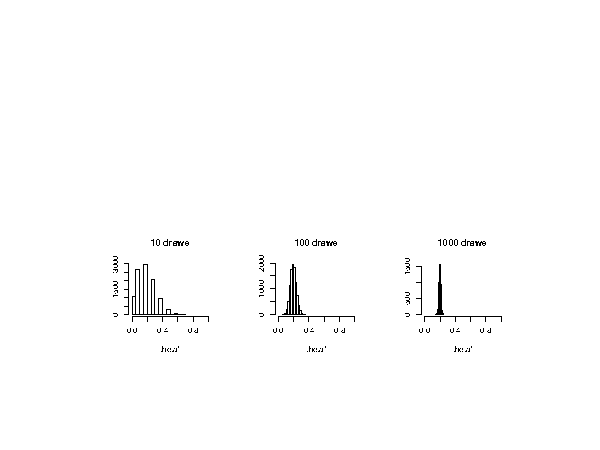
\includegraphics[width=0.9\textwidth]{img/hist-10-100-1000.pdf}
\end{center}

\sld{Estimator Bias}
\begin{itemize}
\item {\bfseries Bias:} expected difference of estimate from true value
\item Continuing previous example
{\small
\begin{Verbatim}
> sims <- rbinom(10000, 1000, 0.2) / 1000
> mean(sims)
[1] 0.2002536
\end{Verbatim}
}
\item Value of 0.2 is estimate of expectation
\item Shows this estimator is \emph{unbiased}
\end{itemize}

\sld{Simple Point Estimation (cont.)}
\begin{itemize}
\item {\bfseries Central Limit Theorem:}  \emph{expected} error in $\theta^*$ goes down as
{\Large
\[
\frac{1}{\sqrt{N}}
\]
}
\item Each decimal place of accuracy requires $100 \times$ more samples.
\item Width of confidence intervals shrinks at the same rate.
\vfill
\item Can also use theory to show this estimator is unbiased.
\end{itemize}

\sld{Pop Quiz! Cancer Clusters}
%
\begin{itemize}
\item Why do lowest and highest cancer clusters look so similar?
\end{itemize}
\vspace*{1pt}
\begin{center}
\hfill
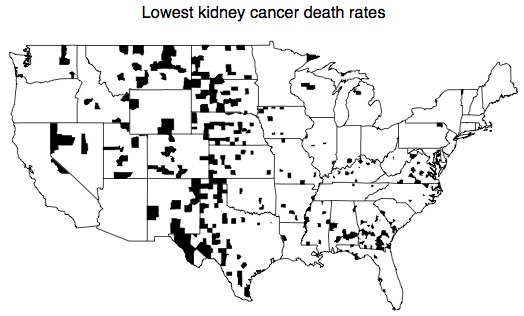
\includegraphics[width=0.45\textwidth]{img/low-cancer.jpg}
\hfill
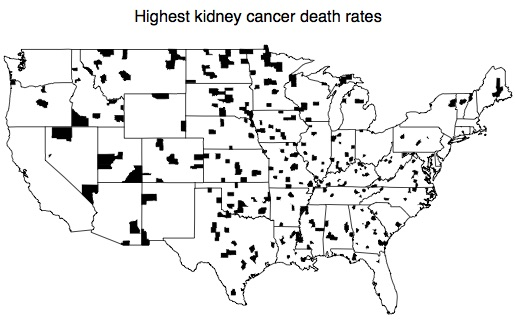
\includegraphics[width=0.45\textwidth]{img/high-cancer.jpg}
\hfill
\end{center}
\vfill
\hfill {\tiny Image from Gelman et al., {\slshape Bayesian Data Analysis, 3rd Edition} (2013)}

\sld{Pop Quiz Answer}
%
\begin{itemize}
\item Hint: mix earlier simulations of repeated i.i.d. trials with 20\% success and sort:
{\footnotesize
\begin{center}
\begin{tabular}{ccccc}
1/10 &  1/10 &  1/10 &  15/100 &  16/100
\\
17/100 &  175/1000 &  179/1000 &  18/100 &  181/1000
\\
188/1000 &  194/1000 &  198/1000 & 2/10 &  2/10 
\\
2/10 &  2/10 & 21/100 &  21/100 &  21/100 
\\
212/1000 &  213/1000 &   216/1000 &   223/1000 &  23/100
\\
26/100 &  26/100 &  3/10 &  4/10 &  5/10 
\end{tabular}
\end{center}
}
\item More variation in observed rates with smaller sample sizes
\vfill
\item \emph{Answer}: High cancer and low cancer counties are small populations
\end{itemize}




\mypart{Warmup Exercise II}{Maximum Likelihood \\[8pt]\spc Estimation}

\sld{Observations, Counterfactuals,
     \\[6pt] \spc{}and Random Variables}
\begin{itemize}
\item Assume we observe data $y = y_1, \ldots, y_N$
\item Statistical modeling assumes even though $y$ is observed,
the values could have been different
\item John Stuart Mill first characterized this {\bfseries counterfactual} nature of statistical modeling in:
\\[3pt] {\slshape A System of Logic, Ratiocinative and Inductive} (1843)
\item In measure-theoretic language, $y$ is a {\bfseries random variable}
\end{itemize}

\sld{Likelihood Functions}
%
\begin{itemize}
\item A \myemph{likelihood function} is a probability function (density, mass, or mixed) 
\[
p(y|\theta,x),
\]
where
\begin{subitemize}
\item $\theta$ is a vector of \myemph{parameters}, 
\item $x$ is some fixed \myemph{unmodeled data} (e.g., regression predictors or
  ``features''),
\item $y$ is some fixed \myemph{modeled data} (e.g., observations)
\end{subitemize}
\item considered as a function $\mathcal{L}(\theta)$ of $\theta$ for fixed $x$ and $y$.
\item can think of as a generative process for $y$how data $y$ is generated
\end{itemize}

\sld{Maximum Likelihood Estimation}
\begin{itemize}
\item \myemph{Estimate} parameters $\theta$ given observations $y$.
\item Maximum likelihood estimation (MLE) chooses 
estimate that maximizes the likelihood function, i.e.,
\[
\theta^* 
\ = \ \argmax_{\theta} \ \mathcal{L}(\theta) 
\ = \ \argmax_{\theta} \ p(y|\theta,x)
\]
\item This function of $\mathcal{L}$ and $y$ (and $x$) is called an \myemph{estimator}
\end{itemize}

\sld{Example of MLE}
%
\begin{itemize}
\item The frequency-based estimate 
\[
\theta^{*} = \frac{1}{N} \sum_{n=1}^N y_n, 
\]
is the observed rate of ``success'' (outcome 1) observations.
\item This is the MLE for the model
\[
p(y|\theta) 
\ = \ \prod_{n=1}^N p(y_n|\theta) 
\ = \  \prod_{n=1}^N \distro{Bernoulli}(y_n|\theta) 
\]
where for $u \in \setcomp{0,1}$, 
{\small
\[
\distro{Bernoulli}(u|\theta) = 
\begin{cases}
\theta & \text{if } u = 1 
\\
1 - \theta & \text{if } u = 0
\end{cases}
\]
}
\end{itemize}

\sld{Example of MLE {\normalsize (cont.)}}
\vspace*{-4pt}
\begin{itemize}
\item First modeling \emph{assumption} is that data are i.i.d.,
\[
p(y|\theta) = \prod_{n=1}^N p(y_n|\theta)
\] 
\item Second modeling \emph{assumption} is form of likelihood,
\[
p(y_n|\theta) = \distro{Bernoulli}(y_n|\theta)
\]
\end{itemize}

\sld{Example of MLE {\normalsize (cont.)}}
\begin{itemize}
\item The frequency-based estimate is the MLE
\item First derivative is zero (indicating min or max),
\[
\mathcal{L}'_y(\theta^*) = 0,
\]
\item Second derivative is negative (indicating max),
\[
\mathcal{L}''_y(\theta^*) < 0.
\]
\end{itemize}

\sld{MLEs can be Dangerous!}
\begin{itemize}
\item Recall the cancer cluster example
\item Accuracy is low with small counts
\item What we need are hierarchical models (stay tuned)
\end{itemize}

\mypart{Part I}{Bayesian Inference}

\sld{Bayesian Data Analysis}
\begin{itemize}
\item ``By {Bayesian data analysis}, we mean {practical methods}
  for making {inferences} from {data} using {probability models}
  for quantities we {observe} and about which we {wish to learn}.''
  % 
\item ``The essential characteristic of Bayesian methods is
  their \myemph{explict use of probability for quantifying uncertainty}
  in inferences based on statistical analysis.''
\end{itemize}
% 
\vfill\hfill{\footnotesize Gelman et al., {\slshape Bayesian Data Analysis},
  3rd edition, 2013}

\sld{Bayesian Methodology}
% 
\begin{itemize}
\item Set up \myemph{full probability model}
  \vspace*{-4pt}
  \begin{itemize}
  \item for all observable \& unobservable quantities
  \item consistent w. problem knowledge \& data collection
  \end{itemize}
  % 
\item \myemph{Condition} on observed data
  \vspace*{-4pt}
  \begin{itemize}
  \item to caclulate posterior probability of unobserved quantities
    (e.g., parameters, predictions, missing data)
  \end{itemize}
  % 
\item \myemph{Evaluate}
  \vspace*{-4pt}
  \begin{itemize}
  \item model fit and implications of posterior
  \end{itemize}
\vfill
\item \myemph{Repeat} as necessary
\end{itemize}

\vfill\hfill {\footnotesize {\slshape Ibid.}}

\sld{Where do Models Come from?}
\begin{itemize}
\item Sometimes model comes first, based on substantive
  considerations
\begin{subitemize}
\item toxicology, economics, ecology, \ldots
\end{subitemize}
\item Sometimes model chosen based on data collection
\begin{subitemize}
\item  traditional statistics of surveys and experiments
\end{subitemize}
\item Other times the data comes first
\begin{subitemize}
\item observational studies, meta-analysis, \ldots
\end{subitemize}
\hfill
\item Usually its a mix
\end{itemize}

\sld{(Donald) Rubin's Philosophy}
\begin{itemize}
\item All statistics is inference about missing data
\item Question 1: What would you do if you had all the data?
\item Question 2: What were you doing before you had any data?
\vfill
\hfill {\footnotesize (as relayed in course notes by Andrew Gelman)}
\end{itemize}

\sld{Model Checking}
\begin{itemize}
\item Do the inferences make sense?
\begin{subitemize}
\item are parameter values consistent with model's prior?
\item does simulating from parameter values produce reasoable fake
  data? 
\item are marginal predictions consistent with the data?
\end{subitemize}
\item Do predictions and event probabilities for new data make sense?
\vfill
\item {\slshape \myemph{Not}}: Is the model true?
\item {\slshape \myemph{Not}}: What is Pr[model is true]?
\item {\slshape \myemph{Not}}: Can we ``reject'' the model?
\end{itemize}

\sld{Model Improvement}
\begin{itemize}
\item Expanding the model
\begin{subitemize}
\item hierarchical and multilevel structure \ldots
\item more flexible distributions (overdispersion, covariance)
\item more structure (geospatial, time series)
\item more modeling of measurement methods and errors
\item \ldots
\end{subitemize}
\item Including more data
\begin{subitemize}
\item breadth (more predictors or kinds of observations)
\item depth (more observations)
\end{subitemize}
\end{itemize}


\sld{Using Bayesian Inference}
\begin{itemize}
\item Finds parameters consistent with prior info and
  data$^*$
\begin{subitemize}
\item $^*$ if such agreement is possible
\end{subitemize}
\item Automatically includes uncertainty and variability
\item Inferences can be plugged in directly
\begin{subitemize}
\item risk assesment
\item decision analysis
\end{subitemize}
\end{itemize}

\sld{Notation for Basic Quantities}
% 
\begin{itemize}
\item \myemph{Basic Quantities}
\begin{subitemize}
\item $y$: \ observed data
\item $\theta$: \ parameters (and other unobserved quantities)
\item $x$: \ constants, predictors for conditional (aka ``discriminative'') models
\end{subitemize}
\item \myemph{Basic Predictive Quantities}
\begin{subitemize}
\item $\tilde{y}$: unknown, potentially observable quantities
\item $\tilde{x}$: \ constants, predictors for unknown quantities
\end{subitemize}
\end{itemize}

\sld{Naming Conventions}

\begin{itemize}
\item \myemph{Joint}: \ $p(y,\theta)$
\item \myemph{Sampling / Likelihood}: \ $p(y|\theta)$
\begin{subitemize}
\item Sampling is function of $y$ with $\theta$ fixed (prob function)
\item Likelihood is function of $\theta$ with $y$ fixed (\emph{not} prob function)
\end{subitemize}
\item \myemph{Prior}: \ $p(\theta)$
\item \myemph{Posterior}: \ $p(\theta|y)$
\item \myemph{Data Marginal (Evidence)}: \ $p(y)$
\item \myemph{Posterior Predictive}: \ $p(\tilde{y}|y)$
\end{itemize}


\sld{Bayes's Rule for Posterior}
% 
\vspace*{-4pt}
\begin{eqnarray*}
    p(\theta|y) 
    & = & \frac{p(y,\theta)}{p(y)} 
          \hspace*{64pt} \text{\small [def of conditional]}
    \\[6pt]
    & = & \frac{p(y|\theta) \, p(\theta)}{p(y)}
          \hspace*{44pt} \text{\small [chain rule]}
    \\[6pt]
    & = & \frac{p(y|\theta) \, p(\theta)}{\int_{\Theta} p(y,\theta') \ d\theta'}
          \hspace*{40pt} \text{\small [law of total prob]}
    \\[6pt]
    & = & \frac{p(y|\theta) \, p(\theta)}{\int_{\Theta} p(y|\theta') \,
      p(\theta') \ d\theta'}
          \hspace*{20pt} \text{\small [chain rule]}
\end{eqnarray*}
\vfill
\begin{itemize}
\item \emph{Inversion:} Final result depends only on 
  sampling distribution (likelihood) $p(y|\theta)$ and prior
  $p(\theta)$
\end{itemize}

\sld{Bayes's Rule up to Proportion}
\begin{itemize}
\item If data $y$ is fixed, then
\begin{eqnarray*}
p(\theta|y) 
& = & \frac{p(y|\theta) \, p(\theta)}{p(y)}
\\[6pt]
& \propto & p(y|\theta) \, p(\theta) 
\\[6pt]
& = & p(y,\theta)
\end{eqnarray*}
\item Posterior proportional to likelihood times prior
\item Equivalently, posterior proportional to joint
\vfill
\item The nasty integral for data marginal $p(y)$ goes away
\end{itemize}

\sld{Posterior Predictive Distribution}
\begin{itemize}
\item Predict new data $\tilde{y}$ based on observed data $y$
\item Marginalize out parameters from posterior
\[
p(\tilde{y}|y)
\ = \
\int_{\Theta} p(\tilde{y}|\theta) \, p(\theta | y) \, d\theta.
\]
\item Averages predictions $p(\tilde{y}|\theta)$,
weight by posterior $p(\theta|y)$
\begin{subitemize}
\item $\Theta = \setcomp{\theta \ | \ p(\theta|y) > 0}$ is support
  of $p(\theta|y)$
\end{subitemize}
\item Allows continuous, discrete, or mixed parameters
\begin{subitemize}
\item integral notation shorthand for sums and/or integrals
\end{subitemize}
\end{itemize}

\sld{Event Probabilities}
\begin{itemize}
\item Recall that an event $A$ is a collection of outcomes
\item Suppose event $A$ is determined by indicator on parameters
\[
f(\theta) 
= 
\begin{cases}
1 & \text{if } \theta \in A
\\
0 & \text{if } \theta \not\in A
\end{cases}
\]
\item e.g., $f(\theta) = \mathrm{I}(\theta_1 > \theta_2)$ 
\ \ for \ \ $\Prob{\theta_1 > \theta_2 \, | \, y}$
\item Bayesian event probabilities calculate posterior mass
\[
\Prob{A} = \int_{\Theta} f(\theta) \, p(\theta|y) \, d\theta.
\]
\item Not frequentist, because involves parameter probabilities
\end{itemize}

\mypart{Example I}{Male Birth Ratio}

\sld{Laplace's Data and Problems}
\begin{itemize}
\item Laplace's data on live births in Paris from 1745--1770: 
\begin{center}\small
\begin{tabular}{c|c}
{\slshape sex} & {\slshape live births}
\\ \hline
female & 241\,945 
\\
male & 251\,527
\end{tabular}
\end{center}
\item Question 1 (Event Probability) 
\\  
Is a boy more likely to be born than a girl?
\item Question 2 (Estimate) 
\\  
What is the birth rate of boys vs. girls?
\item Bayes formulated the basic binomial model
\item Laplace solved the integral
\end{itemize}

\sld{Binomial Distribution}
\begin{itemize}
\item Binomial distribution is number of successes $y$ in $N$ 
i.i.d. Bernoulli trials with chance of success $\theta$
\item If $y_1,\ldots,y_N\sim \distro{Bernoulli}(\theta)$, 
\\[4pt] then $(y_1 + \cdots + y_N) \sim \distro{Binomial}(N,\theta)$
\item The analytic form is
\[
\distro{Binomial}(y|N,\theta) 
\ = \ \binom{N}{y} \theta^{y} (1 - \theta)^{N-y}
\]
where the binomial coefficient normalizes for permutations (i.e.,
which subset of $n$ has $y_n = 1$),
\[
\binom{N}{y} = \frac{N!}{y! \, (N-y)!}
\]
\end{itemize}

\sld{Bayes's Binomial Model}
\begin{itemize}
\item{Data}
\begin{subitemize}
\item $y$: total number of male live births \hfill (data: 241\,945)
\item $N$ : total number of live births \hfill (data: 493\,472)
\end{subitemize}
\item Parameter
\begin{subitemize}
\item $\theta \in (0,1)$: proportion of male live births
\end{subitemize}
\item Likelihood
\[
p(y|N,\theta) 
\ = \ \distro{Binomial}(y|N,\theta) 
\ = \ \binom{N}{y} \theta^{y} (1 - \theta)^{N-y}
\]
\item Prior
\[
p(\theta) 
\ = \ \distro{Uniform}(\theta \, | \, 0,1) 
\ = \ 1
\]
\end{itemize}

\sld{Detour: Beta Distribution}
\begin{itemize}
\item For parameters $\alpha,\beta > 0$ and $\theta \in (0,1)$,
\[
\distro{Beta}(\theta|\alpha,\beta) 
\ \propto \
      \theta^{\alpha - 1} \, 
      (1 - \theta)^{\beta-1}
\]
{\footnotesize
\item Euler's Beta function is used to normalize,
\[
\Betafun(\alpha,\beta) 
\ = \ \int_0^1 u^{\alpha-1}(1-u)^{\beta-1} du
\ = \ \frac{\Gamma(\alpha)\,\Gamma(\beta)}{\Gamma(\alpha + \beta)}
\]
so that
\[
\distro{Beta}(\theta|\alpha,\beta) 
\ = \ \frac{1}{\Betafun(\alpha,\beta)} 
      \theta^{\alpha - 1} \, 
      (1 - \theta)^{\beta-1}
\] 
}
\vfill
\item Note: \ $\distro{Beta}(\theta|1,1) = \distro{Uniform}(\theta|0,1)$
\item Note: $\Gamma()$ is continuous generalization of factorial
\end{itemize}

\sld{Beta Distribution --- Examples}
\vspace*{-4pt}
\begin{itemize}
\item Unnormalized posterior density assuming uniform prior and $y$
  successes out of $n$ trials (all with mean 0.6).
\end{itemize}
\begin{center}
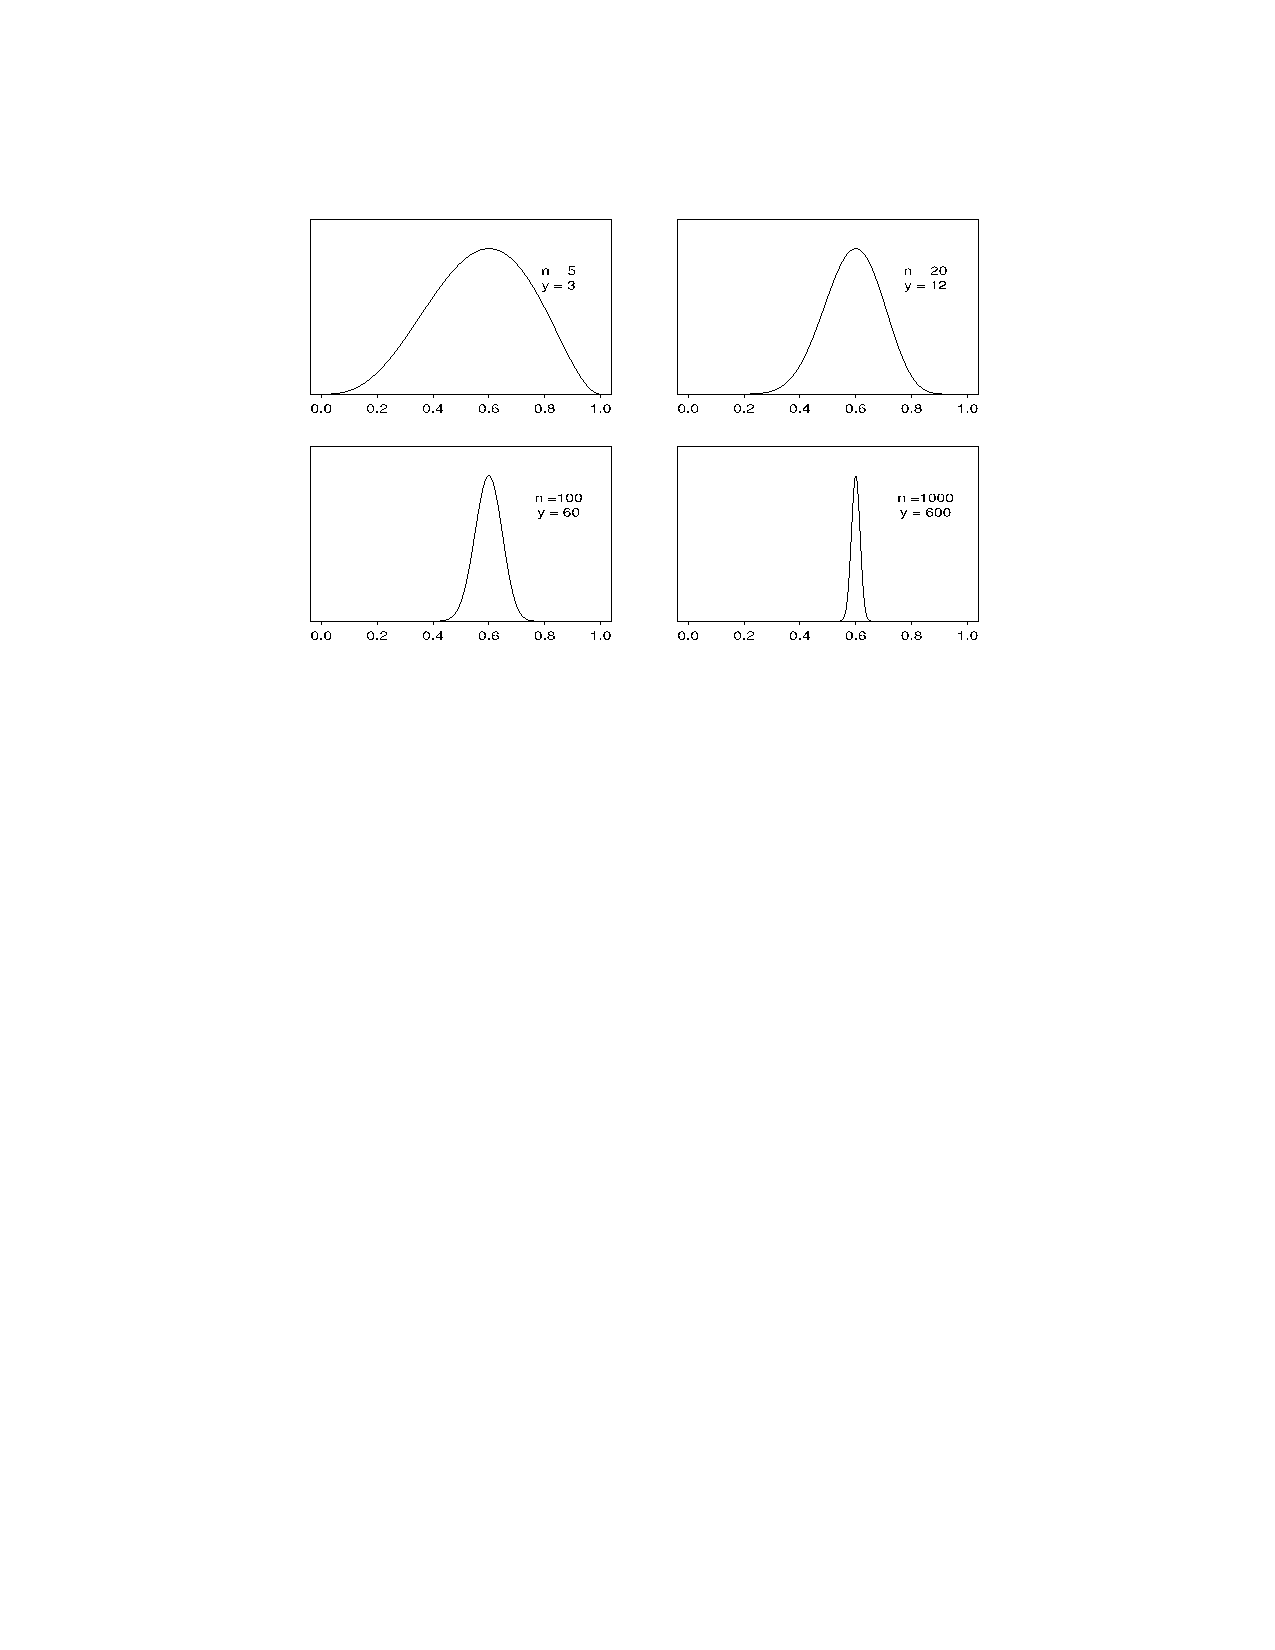
\includegraphics[height=1.6in]{img/bda-beta-plots.pdf}
\end{center}
\vspace*{-12pt}
\hfill {\tiny Gelman et al. (2013) {\slshape Bayesian Data Analysis},
  3rd Edition.}

\sld{Laplace Turns the Crank}
\begin{itemize}
\item From Bayes's rule, the posterior is
\[
p(\theta|y,N) 
\ = \ 
\frac{\distro{Binomial}(y|N,\theta) \, \distro{Uniform}(\theta|0,1)}
     {\int_{\Theta} \distro{Binomial}(y|N,\theta') \,  p(\theta')
       \ d\theta'}
\]
\item Laplace calculated the posterior analytically
\[
p(\theta|y,N) 
\ = \ \distro{Beta}(\theta \, | \, y + 1, \ N - y + 1).
\]
\end{itemize}

\sld{Estimation}
\begin{itemize}
\item Posterior is $\distro{Beta}(\theta \, | \, 1 + 241\,945, \ 1 + 251\,527)$
\item Posterior mean: 
\[
\frac{1 + 241\,945}
     {1 + 241\,945 + 1 + 251\,527}
\approx 0.490291{\bf3}
\]
\item Maximum likelihood estimate same as posterior mode (because
  of uniform prior) 
\[
\frac{241\,945}
     {241\,945 + 251\,527}
\approx 0.490291{\bf2}
\]
\item As number of observations approaches $\infty$, 
\\
MLE approaches posterior mean
\end{itemize}

\sld{Event Probability Inference}
\begin{itemize}
\item What is probability that a male live birth is more likely than a
  female live birth?
\begin{eqnarray*}
\Prob{\theta > 0.5} 
& = &  \int_{\Theta} \indicator{\theta > 0.5} \, p(\theta|y,N) d\theta
\\[4pt]
& = &  \int_{0.5}^1 p(\theta|y,N) d\theta
\\[4pt]
& = &  1 - F_{\theta|y,N}(0.5)
\\[4pt]
& \approx &  10^{-42}
\end{eqnarray*}
\item $\indicator{\phi} = 1$ if condition $\phi$ is true and 0 otherwise.
\item  $F_{\theta|y,N}$ is posterior cumulative distribution
function (cdf).
\end{itemize}

\sld{Mathematics vs.\ Simulation}
\begin{itemize}
\item Luckily, we don't have to be as good at math as Laplace
\item Nowadays, we calculate all these integrals by computer using
  tools like Stan
\vfill
\begin{quote}
  If you wanted to do foundational research in statistics in the
  mid-twentieth century, you had to be bit of a mathematician, whether
  you wanted to or not. \ldots if you want to do statistical research
  at the turn of the twenty-first century, you have to be a computer
  programmer.  \\[3pt] \mbox{ } \hfill {\small ---from Andrew's blog}
\end{quote}
\end{itemize}


\sld{Bayesian ``Fisher Exact Test''}
\vspace*{-4pt}
\begin{itemize}
\item Suppose we observe the following data on handedness
\begin{center}
{\small
\begin{tabular}{c|c|c||c}
     & {\slshape sinister} & {\slshape dexter} & TOTAL
\\ \hline \hline
{\slshape male} & 9 ($y_1$) & 43 & 52 ($N_1$)
\\
{\slshape female} & 4 ($y_2$) & 44 & 48 ($N_2$)
\end{tabular}
}
\end{center}
\item Assume likelihoods $\distro{Binomial}(y_k|N_k,\theta_k)$, uniform
  priors
\item Are men more likely to be lefthanded?
{\small
\begin{eqnarray*}
\Prob{\theta_1 > \theta_2 \, | \, y, N}
& = & 
\int_{\Theta} \indicator{\theta_1 > \theta_2} \, p(\theta|y,N) \, d\theta
\\[8pt]
& \approx &  0.91
\end{eqnarray*}
\item Directly interpretable result; \emph{not} a frequentist procedure
}
\end{itemize}


\sld{Visualizing Posterior Difference}
\begin{itemize}
\item Plot of posterior difference, $p(\theta_1 - \theta_2 \, | \, y,
  N)$ (men - women)
\begin{center}
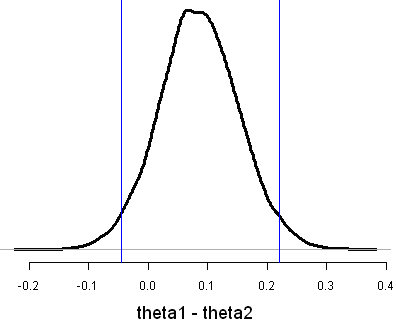
\includegraphics[height=1.5in]{img/bayesian-exact-posterior-handedness.png}
\end{center}
\item Vertical bars: central 95\% posterior interval $(-0.05,0.22)$
\end{itemize}


\mypart{Technical Interlude}{Conjugate Priors}

\sld{Conjugate Priors}
\begin{itemize}
\item Family $\mathcal{F}$ is a conjugate prior for family
  $\mathcal{G}$ if
\begin{subitemize}
\item prior in $\mathcal{F}$ and
\item likelihood in $\mathcal{G}$,
\item entails posterior in $\mathcal{F}$
\end{subitemize}
\item Before MCMC techniques became practical, Bayesian analysis
  mostly involved conjugate priors
\item Still widely used because analytic solutions are more efficient
  than MCMC
\end{itemize}

\sld{Beta is Conjugate to Binomial}
\vspace*{-2pt}
\begin{itemize}
\item Prior: \ \ \ \ \ \ \ \ \ \ \ $p(\theta|\alpha,\beta) =
  \distro{Beta}(\theta|\alpha,\beta)$
\item Likelihood: \ \ $p(y|N,\theta) = \distro{Binomial}(y|N,\theta)$
\item Posterior:
{\small
\begin{eqnarray*}
p(\theta|y,N,\alpha,\beta)
& \propto & p(\theta|\alpha,\beta) \, p(y|N,\theta)
\\[6pt]
& = & \distro{Beta}(\theta|\alpha,\beta) 
      \, \distro{Binomial}(y|N,\theta)
\\
& = & \frac{1}{\Betafun(\alpha,\beta)} 
      \theta^{\alpha - 1} \, 
      (1 - \theta)^{\beta-1}
      \ \
      \binom{N}{y} \theta^{y} (1 - \theta)^{N-y}
\\[6pt]
& \propto & 
      \theta^{y + \alpha - 1} \, 
      (1 - \theta)^{N - y + \beta - 1}
\\[6pt]
& \propto & \distro{Beta}(\theta|\alpha + y, \ \beta + (N - y))
\end{eqnarray*}
}
\end{itemize}

\sld{Chaining Updates}
\vspace*{-4pt}
\begin{itemize}
\item Start with prior $\distro{Beta}(\theta|\alpha,\beta)$
\item Receive binomial data in $K$ statges $(y_1, N_1), \ldots, (y_K, N_K)$
\item After $(y_1,N_1)$, posterior is 
  $\distro{Beta}(\theta|\alpha + y_1, \ \beta + N_1 - y_1)$
\item Use as prior for $(y_2,N_2)$, with posterior \\[3pt]
  $\distro{Beta}(\theta|\alpha + y_1 + y_2, \ \ \beta + (N_1 -
  y_1) + (N_2 - y_2))$
\item Lather, rinse, repeat, until final posterior
\[
\distro{Beta}(\theta|\alpha + y_1 + \cdots + y_K, \ \ \beta + (N_1 +
\cdots + N_K) - (y_1 + \cdots + y_K))
\]
\item Same result as if we'd updated with combined data \\[3pt]
$\distro{Beta}(y_1 + \cdots + y_K, \ \ N_1 + \cdots + N_K)$
\end{itemize}


\mypart{Part II}{(Un-)Bayesian \\[8pt]\spc{}Point Estimation}

\sld{MAP Estimator}
\vspace*{-4pt}
\begin{itemize}
\item For a Bayesian model $p(y,\theta) = p(y|\theta) \, p(\theta)$,
the max a posteriori (MAP) estimate maximizes the posterior,
\begin{eqnarray*}
\theta^{*} 
& = & \argmax_{\theta} \ p(\theta|y)
\\[3pt]
& = & \argmax_{\theta} \ \frac{\displaystyle p(y|\theta) p(\theta)}{p(y)}
\\[3pt]
& = & \argmax_{\theta} \ p(y|\theta) p(\theta).
\\[3pt]
& = & \argmax_{\theta} \ \log p(y|\theta) + \log p(\theta).
\end{eqnarray*}
\item \emph{not} Bayesian because it doesn't integrate over uncertainty
\item \emph{not} frequentist because of distributions over parameters

\end{itemize}

\sld{MAP and the MLE}
\begin{itemize}
\item MAP estimate reduces to the MLE if the prior is uniform, i.e.,
\[
p(\theta) = c
\]
because
\begin{eqnarray*}
\theta^{*} & = & \argmax_{\theta} \ p(y|\theta) \, p(\theta)
\\[4pt]
& = & \argmax_{\theta} \ p(y|\theta) \, c
\\[4pt]
& = & \argmax_{\theta} \ p(y|\theta).
\end{eqnarray*}
\end{itemize}

\sld{Penalized Maximum Likelihood}
\begin{itemize}
\item The MAP estimate can be made palatable to frequentists 
via philosophical sleight of hand 
\item Treat the negative log prior $-\log p(\theta)$ as a ``penalty''
\item e.g., a $\distro{Normal}(\theta|\mu,\sigma)$ prior becomes a penalty function 
\[
\lambda_{\theta, \mu,\sigma}
\  = \ 
-\left( 
   \log \sigma + \frac{1}{2}\left(\frac{\theta -  \mu}{\sigma}\right)^2 
 \right)
\]
\item Maximize sum of log likelihood and negative penalty
\begin{eqnarray*}
\theta^{*} 
& = & \argmax_{\theta} \ \log p(y|\theta,x) - \lambda_{\theta,\mu,\sigma}
\\[4pt]
& = & \argmax_{\theta} \ \log p(y|\theta,x) + \log p(\theta|\mu,\sigma)
\end{eqnarray*}
\end{itemize}

\sld{Proper Bayesian Point Estimates}
\begin{itemize}
\item Choose estimate to minimize some loss function
\item To minimize expected squared error (L2 loss), 
$\expectation{(\theta - \theta')^2 \, | \, y}$, use the posterior mean
\[
\hat{\theta}
\ = \ \argmin_{\theta'} \expectation{(\theta - \theta')^2 \, | \, y}
\ = \ \int_{\Theta} \theta \times p(\theta|y) \, d\theta.
\]
\item To minimize expected absolute error (L1 loss), $\expectation{|\theta -
    \theta'|}$, use the posterior median.
\item Other loss (utility) functions possible, the study of which falls under
  decision theory
\item All share property of involving full Bayesian inference.
\end{itemize}


\sld{Point Estimates for Inference?}
\begin{itemize}
\item Common in machine learning to generate a point estimate
  $\theta^*$, then use it for inference, $p(\tilde{y} | \theta^{*})$
\item This is \myemph{defective} because it
\begin{center}
{\large\myemph{underestimates uncertainty}.}
\end{center}
\item To properly estimate uncertainty, apply full Bayes
\item A major focus of statistics and decision theory is estimating
  uncertainty in our inferences
\end{itemize}

\mypart{Philosophical Interlude}{What is Statistics?}

\sld{Exchangeability}
\begin{itemize}
\item Roughly, an exchangeable probability function is such that for
a sequence of random variables $y = y_1,\ldots,y_N$,
\[
p(y) = p(\pi(y))
\]
for every $N$-permutation $\pi$ (i.e, a one-to-one mapping of $\setcomp{1,\ldots,N}$)
\item i.i.d. implies exchangeability, but not vice-versa
\end{itemize}

\sld{Exchangeability Assumptions}
%
\begin{itemize}
\item Models almost always make some kind of exchangeability assumption
\item Typically when other knowledge is not available
\begin{subitemize}
\item e.g., treat voters as conditionally i.i.d. given their age, 
sex, income, education level, religous affiliation, 
and state of residence
\item But voters have many more properties (hair color, height, profession, employment status, marital status, car ownership, gun ownership, etc.)
\item Missing predictors introduce additional error (on top of measurement error)
\end{subitemize}
\end{itemize}


\sld{Random Parameters:\\[8pt]\spc{}\!Doxastic or Epistemic?}
\begin{itemize}
\item Bayesians treat distributions over parameters as epistemic \\
(i.e., about knowledge) 
\item They do \emph{not} \ treat them as being doxastic \\
(i.e., about beliefs)
\item Priors encode our knowledge before seeing the data
\item Posteriors encode our knowledge after seeing the data
\item Bayes's rule provides the way to update our knowledge
\item People like to pretend models are ontological \\
(i.e., about what exists)
\end{itemize}

\sld{Arbitrariness:\\[8pt]\spc{}\!Priors vs.\ Likelihood}
\begin{itemize}
\item Bayesian analyses often criticized as subjective (arbitrary)
\item Choosing priors is no more arbitrary than choosing a likelihood
  function (or an exchangeability/i.i.d.\ assumption)
\item As George Box famously wrote (1987),
\begin{center}
\large
{\slshape ``All models are wrong, but some are useful.''}
\end{center}
\item This does not just apply to Bayesian models!
\end{itemize}


\mypart{Part IV}{Hierarchical Models}

\sld{Baseball At-Bats}
\begin{itemize}
\item For example, consider baseball batting ability.
\begin{subitemize}
\item 
{\footnotesize Baseball is sort of like cricket, but with round bats, a
  one-way field, stationary ``bowlers'', four bases, short games, 
  and no draws}
\end{subitemize}
\item Batters have a number of ``at-bats'' in a season, out of which they
  get a number of ``hits'' (hits are a good thing)
\item Nobody with higher than 40\% success rate since 1950s.
\item No player (excluding ``bowlers'') bats much less than 20\%.
\item Same approach applies to hospital pediatric surgery
  complications (a BUGS example), reviews on Yelp,
  test scores in multiple classrooms, \ldots
\end{itemize}


\sld{Baseball Data}
\\
%
\begin{minipage}[t]{0.49\textwidth}
\begin{itemize}
\item Hits versus at bats for the 2006 American League season
\item Not much variation in ability!
\item Ignore skill vs. at-bats relation
\item Note uncertainty of MLE
\end{itemize}
\end{minipage}
%
\begin{minipage}[t]{0.50\textwidth}
\begin{center}
\vspace*{-36pt}
\hfill 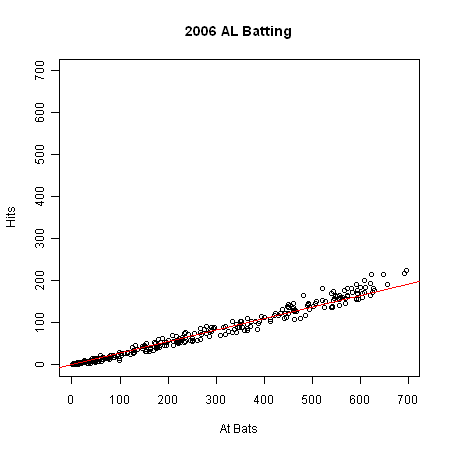
\includegraphics[height=1.4in]{img/al06hitsvsatbats.png}
\\[-18pt]
\hfill 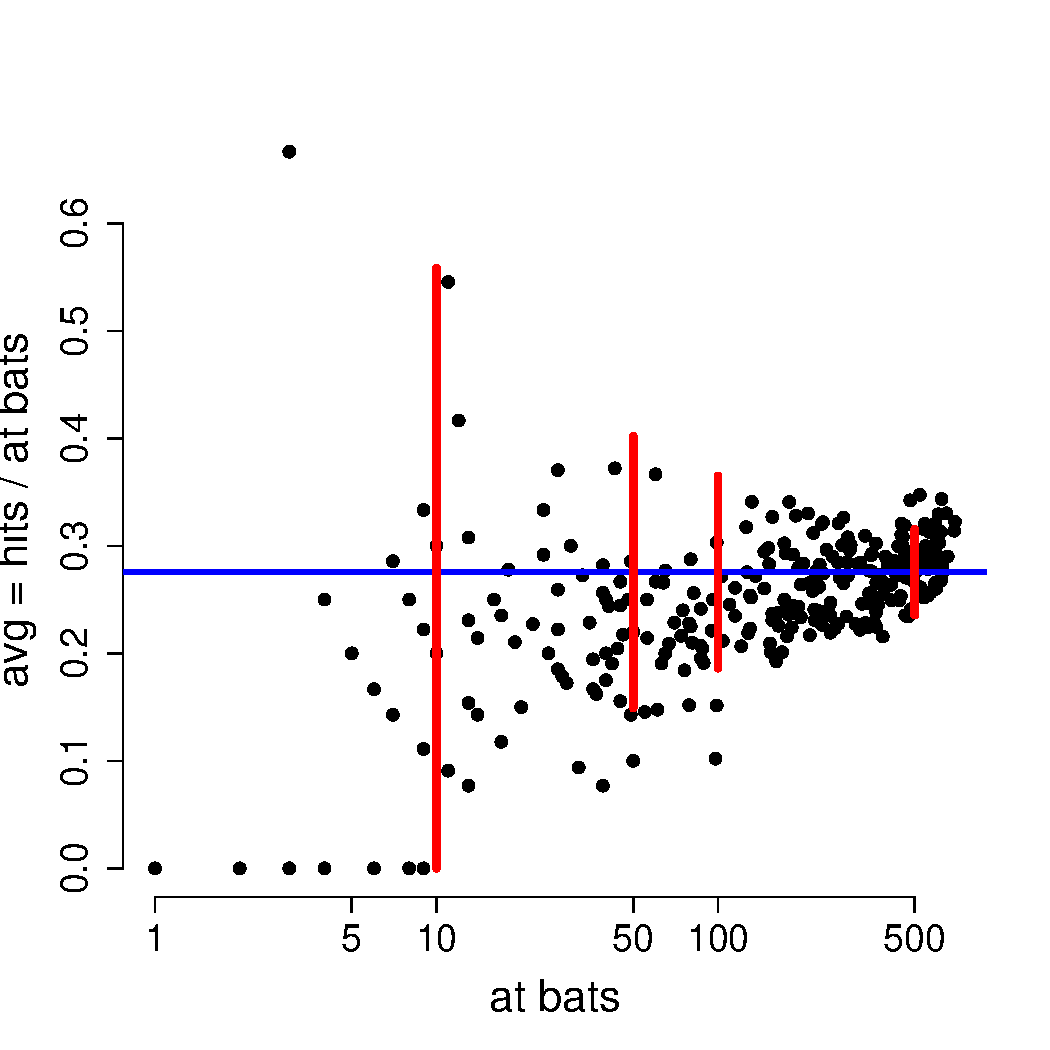
\includegraphics[height=1.4in]{img/bball-eda.pdf}
\end{center}
\end{minipage}

\sld{Pooling Data}
\begin{itemize}
\item How do we estimate the ability of a player who we observe
  getting 6 hits in 10 at-bats?  Or 0 hits in 5 at-bats?  Estimates of
  60\% or 0\% are absurd!
\item Same logic applies to players with 152 hits in 537 at bats.
\item \emph{No pooling}: estimate each player separately
\item \emph{Complete pooling}: estimate all players together (assume no difference
  in abilities)
\item \emph{Partial pooling}: somewhere in the middle
\begin{subitemize}
\item use information about other players (i.e., the population) 
to estimate a player's ability
\end{subitemize}
\end{itemize}

\sld{Hierarchical Models}
\begin{itemize}
\item Hierarchical models are principled way of determining how much
  pooling to apply.
\item Pull estimates toward the population mean based on amount of
  variation in population
\begin{subitemize}
\item low variance population: more pooling
\item high variance population: less pooling
\end{subitemize}
\item In limit
\begin{subitemize}
\item as variance goes to 0, get complete pooling
\item as variance goes to $\infty$, get no pooling
\end{subitemize}
\end{itemize}

\sld{Hierarchical Batting Ability}
\begin{itemize}
\item Instead of fixed priors, estimate priors along with other parameters
\item Still only uses data once for a single model fit
\item Data: $y_n, B_n$: hits, at-bats for player $n$
\item Parameters: $\theta_n$: ability for player $n$
\item Hyperparameters: $\alpha, \beta$: population mean and variance
\item Hyperpriors: fixed priors on $\alpha$ and $\beta$ (hardcoded)
\end{itemize}

\sld{Hierarchical Batting Model {\small (cont.)}}
\vspace*{-4pt}
\begin{eqnarray*}
y_n & \sim & \distro{Binomial}(B_n, \theta_n)
\\[4pt]
\theta_n & \sim & \distro{Beta}(\alpha,\beta)
\\[4pt]
\frac{\alpha}{\alpha + \beta} & \sim & \distro{Uniform}(0,1)
\\[4pt]
(\alpha + \beta) & \sim & \distro{Pareto}(1.5)
\end{eqnarray*}
\begin{itemize}
\item Sampling notation syntactic sugar for: \\[4pt]
{\footnotesize 
$
p(y,\theta,\alpha,\beta)
\ = \
\distro{Pareto}(\alpha + \beta | 1.5)
\,
\prod_{n=1}^N 
  \Big(
  \distro{Binomial}(y_n|B_n, \theta_n)
  \
  \distro{Beta}(\theta_n|\alpha,\beta) 
  \Big)
$
}
\item Pareto provides power law: \ \
{\small 
$
\distro{Pareto}(u|\alpha) \propto
\frac{\alpha}{u^{\alpha + 1}}
$
}
\item Should use more informative hyperpriors!
\end{itemize}

\sld{Hierarchical Prior Posterior}
\\[8pt]
\begin{minipage}[t]{0.55\textwidth}
\begin{itemize}
\item Draws from posterior (crosshairs at posterior mean)
\item Prior population mean:   0.271
\item Prior population scale:  400
\item Together yield prior std dev of 0.022
\item Mean is better estimated than scale (typical)
\end{itemize}
\end{minipage}
\begin{minipage}[t]{0.45\textwidth}
\vfill
\mbox{ } \ \ \ \ \ \ 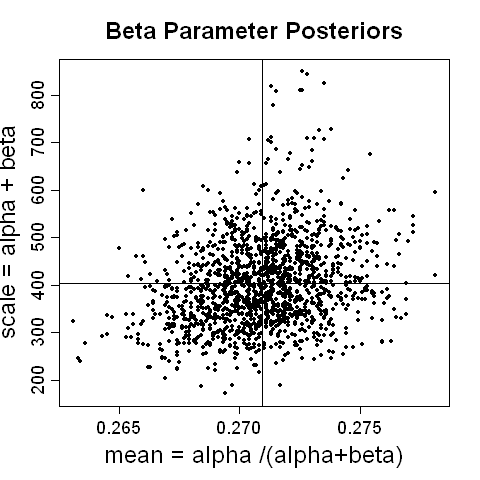
\includegraphics[height=1.4in]{img/baseball-beta-posterior-scatter.png}
\vfill
\end{minipage}

\sld{Posterior Ability {\normalsize (High Avg Players)}}
\\[8pt]
\begin{minipage}[t]{0.45\textwidth}
\begin{itemize}
\item Histogram of posterior draws for high-average players
\item Note uncertainty grows with lower at-bats
\\
\end{itemize}
\end{minipage}
\begin{minipage}[t]{0.55\textwidth}
\vfill
\mbox{ } \ \ \ \ \ \ 
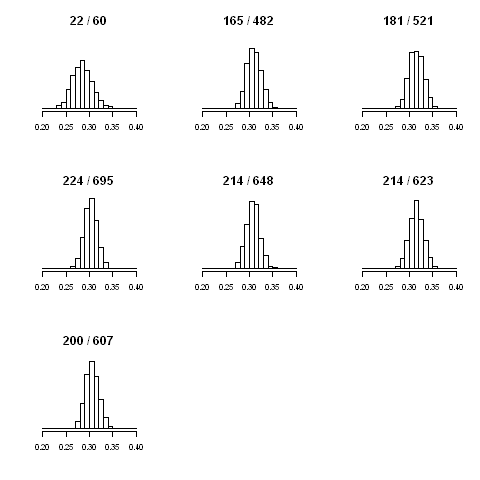
\includegraphics[height=1.95in]{img/batting-ability-posteriors.png}
\vfill
\end{minipage}

\sld{Multiple Comparisons}
\vspace*{-2pt}\small
\begin{itemize}
\item Who has the highest ability (based on this data)?
\item Probabilty player $n$ is best is 
\end{itemize}
%
\begin{center}
{\small
\begin{tabular}{rrr}
\emph{Average} & \emph{At-Bats} & $\Prob{\text{best}}$
\\ \hline
.347 & 521 & 0.12
\\
.343 & 623 & 0.11
\\
.342 & 482 & 0.08
\\
.330 & 648 & 0.04
\\
.330 & 607 & 0.04
\\
.367 & 60 & 0.02
\\
.322 & 695 & 0.02
\end{tabular}
}
\end{center}
\begin{itemize}
\item No clear winner---sample size matters.
\item In last game (of 162), Mauer (Minnesota) edged out Jeter (NY)
\end{itemize}

\mypart{}{End (Section 1)}

\end{document}

